\section{Introduction to Laboratory Practice} 

\begin{multicols}{2}


%==================================================================================================%

\section*{Laboratory Rules and Safety} \index{Laboratory! rules and safety}


\subsection[Display of Hazardous Chemicals]{Display of Hazardous \hfill \\ Chemicals}

\begin{center}
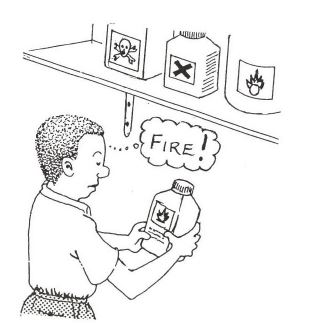
\includegraphics[width=0.45\textwidth]{./img/source/display-chemicals.jpg}
\end{center}

\begin{description*}
%\item[Subtopic:]{}
%\item[Materials:]{}
%\item[Setup:]{}
\item[Procedure:]{Display some well labelled containers with
hazard symbols for the students and let them
talk about them.}
%\item[Hazards:]{}
%\item[Questions:]{}
%\item[Observations:]{}
%\item[Theory:]{}
%\item[Applications:]{}
%\item[Notes:]{}
\end{description*}

\subsection{A Safety Game}

\begin{center}
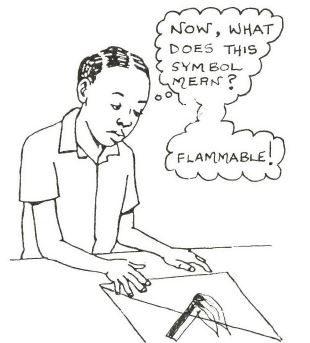
\includegraphics[width=0.45\textwidth]{./img/source/safety-game.jpg}
\end{center}

\begin{description*}
%\item[Subtopic:]{}
\item[Materials:]{Cards of hazard symbols}
%\item[Setup:]{}
\item[Procedure:]{Play a game with the symbol charts. A
student is given a hazard symbol. He has to
explain the hazard shown and to explain the
necessary safety precautions in order to avoid
that hazard.}
%\item[Hazards:]{}
%\item[Questions:]{}
%\item[Observations:]{}
%\item[Theory:]{}
%\item[Applications:]{}
%\item[Notes:]{}
\end{description*}

\columnbreak

\subsection{The Cleanliness Play}

\begin{center}
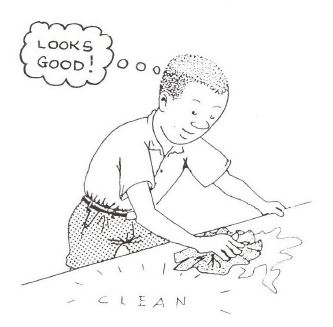
\includegraphics[width=0.45\textwidth]{./img/source/cleanliness-play.jpg}
\end{center}

\begin{description*}
%\item[Subtopic:]{}
%\item[Materials:]{}
%\item[Setup:]{}
\item[Procedure:]{Ask the students to play group-wise short
and funny scenes using appropriate words to
make them familiar with cleanliness rules.}
%\item[Hazards:]{}
%\item[Questions:]{}
%\item[Observations:]{}
%\item[Theory:]{}
%\item[Applications:]{}
%\item[Notes:]{}
\end{description*}

\subsection{The Tidiness Play}

\begin{center}
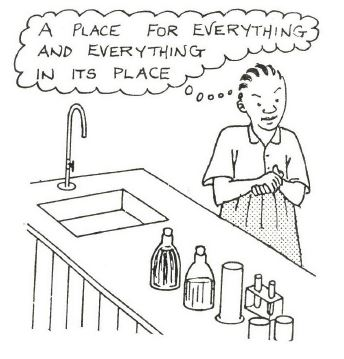
\includegraphics[width=0.45\textwidth]{./img/source/tidiness-play.jpg}
\end{center}

\begin{description*}
%\item[Subtopic:]{}
%\item[Materials:]{}
%\item[Setup:]{}
\item[Procedure:]{Chemists are very tidy. Apparatus and
reagents should be arranged on the table so that
they can be reached easily but at a safe distance
from the experiment.}
%\item[Hazards:]{}
%\item[Questions:]{}
%\item[Observations:]{}
%\item[Theory:]{}
%\item[Applications:]{}
%\item[Notes:]{}
\end{description*}

\end{multicols}

\pagebreak

%==================================================================================================%

\section*{The Scientific Method} \index{Scientific method}
\label{sec:scientific-method}

%\setcounter{secnumdepth}{1}

The following activities can be used as a method of introducing students to the scientific method. Rather than just performing the activities, first identify the question or problem with the students, then have them form a hypothesis for each step of the experiment. Students should record observations and data accordingly and use them to draw a conclusion about the activity.\\

Prepare an activity sheet for each student or have them copy it into their notebooks before performing the activities. Set up stations for the various activities and have students rotate among them in small groups. Incorporate activities in Biology and Chemistry as well from the \emph{Shika na Mikono} resource manual.\\


\subsection{Complete the Circuit} \index{Electricity! current}

\begin{center}
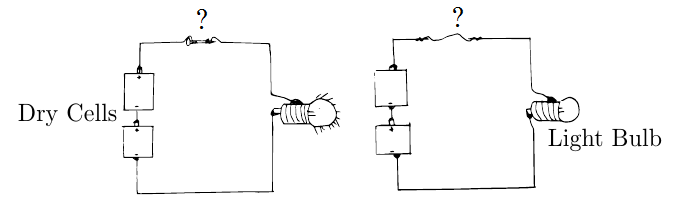
\includegraphics[width=0.8\textwidth]{./img/conductors-insulators-sci-meth.png}
\end{center}

\begin{description*}
\item[Materials:]{Dry cell, speaker wire, bulb/ammeter, cardboard, various objects, e.g. rubber band, nail, paper, aluminum foil, toothpick, pen, scissors, bottle cap, coin, balloon, chalk}
\item[Setup:]{Connect a dry cell and bulb in series using speaker wire and attach to a sheet of cardboard. Leave two wires free and pin to the cardboard to act as a switch.}
\item[Problem:]{Which objects will light a bulb?\\

\begin{tabular}{|l|c|c|} \hline
\multirow{2}{*}{\textbf{Object}} & \textbf{Hypothesis} & \multirow{2}{*}{\textbf{Experimental Result}} \\
& \textbf{(Light or No Light)} & \\ \hline
Copper wire & & \\ \hline
Pen & & \\ \hline
Aluminum foil& & \\ \hline
Paper& & \\ \hline
Nail& & \\ \hline
Toothpick& & \\ \hline
Bottle cap& & \\ \hline
Balloon& & \\ \hline
Chalk& & \\ \hline
Scissors (blade)& & \\ \hline
Scissors (handle)& & \\ \hline
\end{tabular}\\[10pt]
}
\item[Hypothesis:]{Predict which materials will cause the bulb to light when placed across the switch. Record predictions in the table.}
\item[Procedure:]{Test each object by placing it across the free wires to close the circuit.}
\item[Observations:]{Record the result for each item in the table.}
\item[Questions:]{}\hfill 
\begin{enumerate}
\item Which materials caused the bulb to light?
\item These objects are made from what kind or materials?
\item What other objects in the room can you find to test? Will they light the bulb?
\end{enumerate}
\item[Theory:]{\emph{Conductors} are materials which easily allow electrons to flow through them. \emph{Insulators} are materials which do not easily allow the the flow of electrons. Examples of good conductors are most metals, water and the human body. Examples of good insulators are rubber, wood and plastic.}
\end{description*}

\pagebreak


\subsection{Density Tower} \index{Density}

\begin{center}
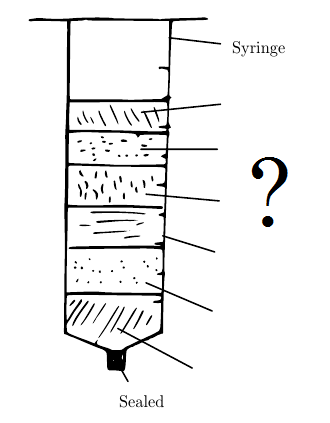
\includegraphics[width=0.3\textwidth]{./img/density-tower-sci-meth.png}
\end{center}

\begin{description*}
\item[Materials:]{Syringes, bottles, water, cooking oil, kerosene, spirit, honey, glycerine, tape, scissors}
\item[Setup:]{Prepare a test tube rack by cutting a bottle and filling it with dirt. Remove the plungers from the syringes and seal them with tape, super glue, or by melting to opening closed.}\\
\item[Problem:]{Which liquids are more dense than others?\\

\begin{tabular}{|l|c|c|} \hline
\multirow{2}{*}{\textbf{Liquid}} & \textbf{Hypothesis} & \multirow{2}{*}{\textbf{Experimental Result}} \\
& \textbf{(Position, 1 = bottom)} & \\ \hline
Water & & \\ \hline
Cooking oil & & \\ \hline
Kerosene & & \\ \hline
Spirit & & \\ \hline
Honey & & \\ \hline
Glycerine & & \\ \hline
\end{tabular} \\[10pt]
}\\
\item[Hypothesis:]{Predict the order in which the liquids will settle from the bottom of the syringe. Assign 1 to the bottom liquid, 2 to the one above it, and so on.}
\item[Procedure:]{Pour a small amount of each liquid into a syringe, observing after each addition.}
\item[Observations:]{After adding all liquids, record the order in which they rest, starting with 1 at the bottom.}
\item[Questions:]{}\hfill
\begin{enumerate}
\item Which liquid finished at the bottom?
\item Which liquid finished at the top?
\item Which liquid has the greatest density?
\item Which liquid has the lowest density?
\item What happens if you place a small object (e.g. paper clip, eraser, paper) in the tower? 
\end{enumerate}
\item[Theory:]{\emph{Density} is a property of different materials and liquids. It is a ratio of its mass to its volume. Dense liquids sink to the bottom, while less dense liquids rise to the top. A small object placed in the tower will settle in the liquid which is nearest its own density.}
\end{description*}

\pagebreak


\subsection{Sinkers and Floaters} \index{Flotation}

%\begin{center}
%\includegraphics[width=0.4\textwidth]{./img/source/.jpg}
%\end{center}

\begin{description*}
\item[Materials:]{Basin of water, various objects, e.g. nail, paper clip, paper, aluminum foil, soda cap, matchbox, pen cap, toothpick, balloons, flour}
%\item[Setup:]{}\\
\item[Problem:]{Which objects sink or float when placed in water?\\

\begin{tabular}{|l|c|c|} \hline
\multirow{2}{*}{\textbf{Object}} & \textbf{Hypothesis} & \multirow{2}{*}{\textbf{Experimental Result}} \\
& \textbf{(Sink or Float)} & \\ \hline
Nail& & \\ \hline
Paper clip& & \\ \hline
Pen cap& & \\ \hline
Soda cap (dropped)& & \\ \hline
Soda cap (placed carefully)& & \\ \hline
Toothpick & & \\ \hline
Paper& & \\ \hline
Aluminum foil& & \\ \hline
Matchbox& & \\ \hline
Balloon (empty)& & \\ \hline
Balloon (filled with flour)& & \\ \hline
Balloon (filled with water)& & \\ \hline
Balloon (filled with air)& & \\ \hline
\end{tabular} \\[10pt]
}\\
\item[Hypothesis:]{Predict whether each object will sink or float when placed in the basin of water. Record in the table.}
\item[Procedure:]{Place each object in the water. First place them very carefully, then drop them in.}
\item[Observations:]{Record the results in the table.}
\item[Questions:]{}\hfill
\begin{enumerate}
\item What factors affect whether an object sinks or floats?
\item How do large objects such as boats float?
\end{enumerate}
\item[Theory:]{\emph{Flotation} depends on several things. A bottle cap placed carefully on the surface of the water will float, but when pushed under, will sink. A sheet of aluminum foil will float while a sheet of the same size which is folded several times will sink. A balloon filled with flour sinks, one filled with water just floats, and one filled with air floats above the surface.\\

If an object's \emph{total density} is greater than that of water, it sinks, but if less than water, it floats. Air has a density less than water, so when air is trapped in objects such as bottle caps or balloons, they float because their total density is less than water. When air is removed (folded aluminum foil) or replaced by water (bottle cap), the total density of the object is just the density of the material. A matchbox pushed under water rises back to the surface because its density is less than that of water.\\

Boats are able to float despite being built from dense materials because of the large volume of water they displace and the large amount of air inside the boat. A boat with a larger surface area displaces a larger volume of water and thus can carry a larger load before sinking.\\

Follow up this activity with the \emph{Raft Rally} science competition.}
\end{description*}

\pagebreak


\subsection{Mixing Colours} \index{Colour}

%\begin{center}
%\includegraphics[width=0.4\textwidth]{./img/source/.jpg}
%\end{center}

\begin{description*}
\item[Materials:]{Various food colours, syringes, bottle, scissors, tape, paper}
\item[Setup:]{Prepare a test tube rack by cutting a bottle and filling it with dirt. Remove the plungers from the syringes and seal them with tape, super glue, or by melting to opening closed.}\\
\item[Problem:]{What happens when we mix different colours?\\

\begin{tabular}{|l|c|c|} \hline
\multirow{2}{*}{\textbf{Colours to Mix}} & \textbf{Hypothesis} & \multirow{2}{*}{\textbf{Experimental Result}} \\
& \textbf{(What colour?)} & \\ \hline
Red and green & & \\ \hline
Yellow and blue & & \\ \hline
Red and yellow & & \\ \hline
All colours & & \\ \hline
\end{tabular} \\[10pt]
}\\
\item[Hypothesis:]{Predict which colour will result when the two colours given are mixed together. Record it in the table.}
\item[Procedure:]{Use syringes to remove small amounts of each colour and place on a sheet of paper. Be sure to lay down plenty of paper so that the colours do not bleed through onto the table!}
\item[Observations:]{Record the resulting colour mixture in the table.}
\item[Questions:]{}\hfill
\begin{enumerate}
\item How can you make orange from other colours?
\item What colour do you get by mixing all of the colours together?
\item What are some uses of coloured dyes?
\end{enumerate}
\item[Theory:]{Red, green and blue are \emph{primary colours} of light. Other colours are made by different combinations of these primary colours. Coloured dyes are used for many applications, including clothes, paper and printing pictures.}
\end{description*}

%==================================================================================================%

%\setcounter{secnumdepth}{2}

%\end{multicols}
\vfill
\pagebreak